\documentclass{article} % For LaTeX2e
\usepackage{nips14submit_e,times}
\usepackage{amsmath}
\usepackage{amsthm}
\usepackage{amssymb}
\usepackage{mathtools}
\usepackage{hyperref}
\usepackage{url}
\usepackage{algorithm}
\usepackage[noend]{algpseudocode}
%\documentstyle[nips14submit_09,times,art10]{article} % For LaTeX 2.09

\usepackage{mathrsfs}
\usepackage{graphicx}
\usepackage{caption}
\usepackage{subcaption}

\def\eQb#1\eQe{\begin{eqnarray*}#1\end{eqnarray*}}
\def\aB#1\aE{\begin{align*}#1\end{align*}}
\def\eQnb#1\eQne{\begin{align}#1\end{align}}
\providecommand{\e}[1]{\ensuremath{\times 10^{#1}}}
\providecommand{\pb}[0]{\pagebreak}

\newcommand{\E}{\mathrm{E}}
\newcommand{\Var}{\mathrm{Var}}
\newcommand{\Cov}{\mathrm{Cov}}

\def\Qb#1\Qe{\begin{question}#1\end{question}}
\def\Sb#1\Se{\begin{solution}#1\end{solution}}

\usepackage{scalerel,stackengine}
\stackMath
\newcommand\reallywidehat[1]{%
\savestack{\tmpbox}{\stretchto{%
  \scaleto{%
    \scalerel*[\widthof{\ensuremath{#1}}]{\kern-.6pt\bigwedge\kern-.6pt}%
    {\rule[-\textheight/2]{1ex}{\textheight}}%WIDTH-LIMITED BIG WEDGE
  }{\textheight}% 
}{0.5ex}}%
\stackon[1pt]{#1}{\tmpbox}%
}

\newenvironment{claim}[1]{\par\noindent\underline{Claim:}\space#1}{}
\newtheoremstyle{quest}{\topsep}{\topsep}{}{}{\bfseries}{}{ }{\thmname{#1}\thmnote{ #3}.}
\theoremstyle{quest}
\newtheorem*{definition}{Definition}
\newtheorem*{theorem}{Theorem}
\newtheorem*{lemma}{Lemma}
\newtheorem*{question}{Question}
\newtheorem*{preposition}{Preposition}
\newtheorem*{exercise}{Exercise}
\newtheorem*{challengeproblem}{Challenge Problem}
\newtheorem*{solution}{Solution}
\newtheorem*{remark}{Remark}
\usepackage{verbatimbox}
\usepackage{listings}
\title{Harmonic Analysis:  \\
Problem Set V}


\author{
Youngduck Choi \\
CIMS \\
New York University\\
\texttt{yc1104@nyu.edu} \\
}


% The \author macro works with any number of authors. There are two commands
% used to separate the names and addresses of multiple authors: \And and \AND.
%
% Using \And between authors leaves it to \LaTeX{} to determine where to break
% the lines. Using \AND forces a linebreak at that point. So, if \LaTeX{}
% puts 3 of 4 authors names on the first line, and the last on the second
% line, try using \AND instead of \And before the third author name.

\newcommand{\fix}{\marginpar{FIX}}
\newcommand{\new}{\marginpar{NEW}}

\nipsfinalcopy % Uncomment for camera-ready version

\begin{document}


\maketitle

\begin{abstract}
This work contains solutions to the problem set IV
of Harmonic Analysis 2016 at Courant Institute of Mathematical Sciences.
\end{abstract}

\bigskip

\begin{question}[1]
\hfill
\begin{figure}[h!]
  \centering
    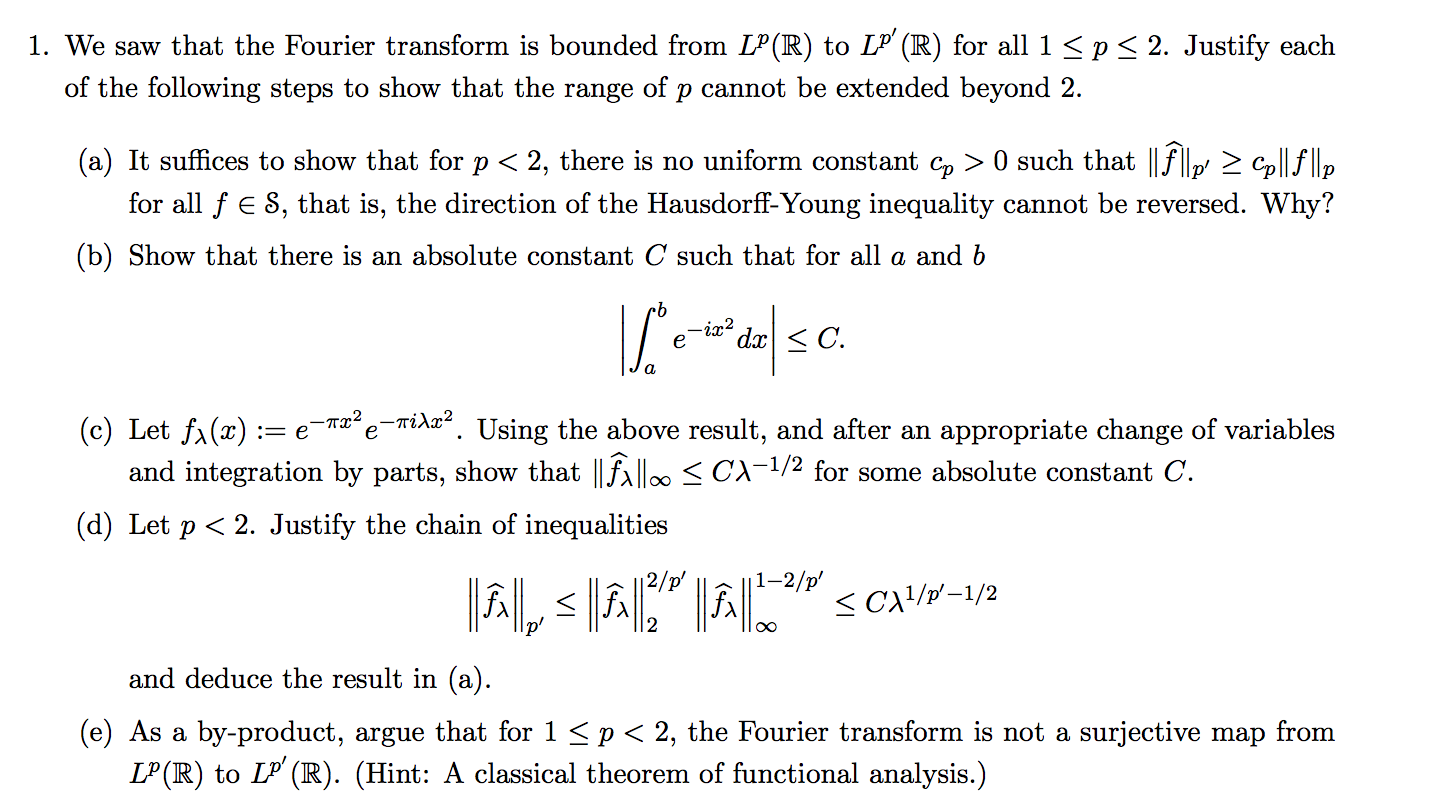
\includegraphics[width=0.8\textwidth]{HA-5-1.png}
\end{figure}
\end{question}
\begin{solution} \hfill \\
\textbf{(a)}
Let $p < 2$.
Assume that there is no uniform constant $c_p > 0$ such that $||\hat{f}||_{p'} \geq 
c_p ||f||_{p}$ for all $f \in S$. Since Fourier transform is a bijective mapping
from $S$ to $S$, and, for $f \in S$, $||\hat{\hat{f}}||_{p'} = ||f||_{p'}$ (Fourier transform
composed twice on the Schwarz space is a parity operator, which does not change
any $L^p$ norm for $f \in S$), substituting $\hat{f}$
in the position of $f$ implies that there is no uniform constant $c_p > 0$ such that 
\eQb
||f||_{p'} &\geq& c_p ||\hat{f}||_{p}, 
\eQe
for any $f \in S$. Since $S \subset L^p$, we conclude that the given statement is sufficient.

\bigskip

\textbf{(b)} With $u = \sqrt{i}x$, it follows that
\eQb
\int e^{ix^2} = \dfrac{1}{\sqrt{i}} \int e^{u^2} du = (\dfrac{1}{\sqrt{2}}
- i \dfrac{1}{\sqrt{2}} )\text{erf} (u) + C, 
\eQe
where the last equality holds with the well-known error function. Since $|\text{erf}(z)| \leq 1$ 
for any $z \in \mathbb{C}$, it follows that
\eQb
|\int_{a}^{b} e^{ix^2} dx| &=& 
|(\dfrac{1}{\sqrt{2}} - i\dfrac{1}{\sqrt{2}})|
|\text{erf}(b) - \text{erf}(a)| \\ 
&\leq&  2|(\dfrac{1}{\sqrt{2}} - i\dfrac{1}{\sqrt{2}})| \leq C,
\eQe
for some absolute constant $C$.

\bigskip

\textbf{(c)} With $y = \sqrt{\pi \lambda}x$, we compute with integration by parts
\eQb
|\hat{f_{\lambda}}(\xi)| &=& 
 |\int_{\mathbb{R}} e^{-(\frac{y-\xi\sqrt{\frac{\pi}{\lambda}}}{2})^2} e^{-iy^2} dy| \\
&\leq& 
|\int_{\xi\sqrt{\frac{\pi}{\lambda}}}^{\infty}
 e^{-(\frac{y-\xi\sqrt{\frac{\pi}{\lambda}}}{2})^2} e^{-iy^2} dy| \\
&+& |\int_{-\infty}^{\xi\sqrt{\frac{\pi}{\lambda}}}
 e^{-(\frac{y-\xi\sqrt{\frac{\pi}{\lambda}}}{2})^2} e^{-iy^2} dy| \\
&=& |\int_{\xi\sqrt{\frac{\pi}{\lambda}}}^{\infty}
 2(\dfrac{y-\xi\sqrt{\frac{\pi}{\lambda}}}{\lambda})\dfrac{1}{\lambda}
e^{-(\frac{y-\xi\sqrt{\frac{\pi}{\lambda}}}{2})^2} F(y) dy| \\
&+& |\int_{-\infty}^{\xi\sqrt{\frac{\pi}{\lambda}}}
2(\dfrac{y-\xi\sqrt{\frac{\pi}{\lambda}}}{\lambda})\dfrac{1}{\lambda}
 e^{-(\frac{y-\xi\sqrt{\frac{\pi}{\lambda}}}{2})^2} F(y) dy| \leq C,\\
\eQe 
for some absolute constant $C$,
so
\eQb
||\hat{f}_{\lambda}||_{\infty} \leq C\lambda^{-\frac{1}{2}}, 
\eQe
as required.

\bigskip

\textbf{(d)} By generalized Holder's inequality with $n = 2$ and $\theta = \frac{2}{p'}$, we obtain
\eQb
||\hat{f}_{\lambda}||_{p'} &\leq& ||\hat{f}_{\lambda}||_{2}^{\frac{2}{p'}} 
||\hat{f}_{\lambda}||_{\infty}^{1-\frac{2}{p'}}.
\eQe

As $|e^{-\pi i \lambda x^2}| = 1$ for any $x \in \mathbb{R}$, and $||f||_{2} = ||\hat{f}||_{2}$ for $f 
\in L^2$,  
we see that
\eQb
||\hat{f}_{\lambda}||_{2} &=& ||f_{\lambda}||_{2} = 
(\int_{\mathbb{R}} |e^{-\pi x^2}e^{-\pi i \lambda x^2}|^p)^{\frac{1}{p}} 
= ||e^{-\pi x^2}||_{p} = C, 
\eQe
for some absolute constant $C$. Therefore, by $(c)$ and the above equality, it follows that
\eQb
||\hat{f}_{\lambda}||_{p'} &\leq& ||\hat{f}_{\lambda}||_{2}^{\frac{2}{p'}} 
||\hat{f}_{\lambda}||_{\infty}^{1-\frac{2}{p'}} \leq C\lambda^{\frac{1}{p'}-\frac{1}{2}},
\eQe
for some absolute constant $C$. Now, we deduce $(a)$. Similarly, we have
\eQb
||f_{\lambda}||_{p} &=& (\int_{\mathbb{R}} |e^{-\pi x^2}e^{-\pi i \lambda x^2}|^p)^{\frac{1}{p}} 
= ||e^{-\pi x^2}||_{p} = \delta, 
\eQe
for some constant $\delta > 0$, independent of $\lambda$.
 Let $c_p > 0$ be given. Then, for $\lambda > 0$ sufficiently small, it follows that
\eQb
||\hat{f}_{\lambda}||_{p'} \leq C\lambda^{\frac{1}{p'}-\frac{1}{2}} \leq c_p ||f_{\lambda}||_{p}, 
\eQe
where $C$ is some absolute constant. Therefore, there does not exist a uniform constant $c_p > 0$
such that $||\hat{f}||_{p'} \geq c_p ||f||_{p}$ for all $f \in S$.

\bigskip


\textbf{(e)} Let $1 \leq p < 2$.
Suppose for sake of contradiction that Fourier transform is a surjective 
map from $L^p$ to $L^{p'}$. As the Fourier 
transform is unique on $L^p$ for $1 \leq p < 2$, this implies that the Fourier transform is a 
bijective map from $L^p$ to  $L^{p'}$. Now, by the Open Mapping theorem, we have that
the Fourier transform is a bijective, open map from $L^p$ to $L^{p'}$. Then,
the inverse map of the Fourier transform is well-defined and continuous from $L^{p'}$
to $L^p$. This is a contradiction to $(a)$.

\end{solution}

\newpage

\begin{question}[2]
\hfill
\begin{figure}[h!]
  \centering
    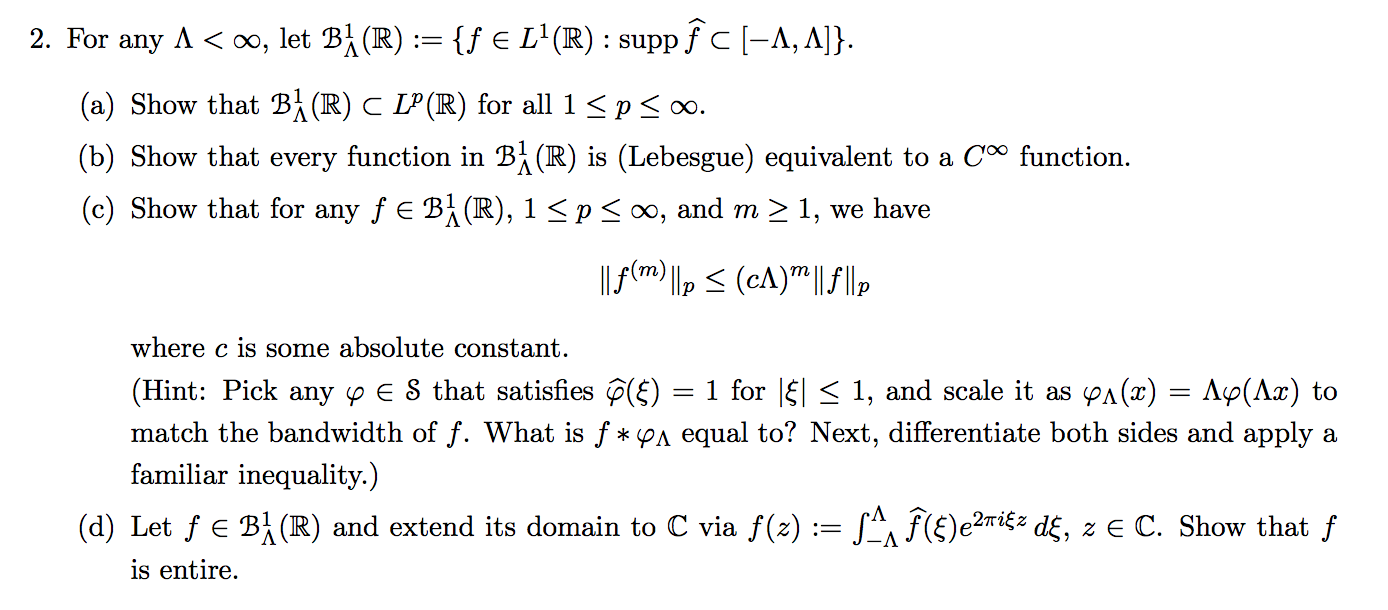
\includegraphics[width=0.8\textwidth]{HA-5-2.png}
\end{figure}
\end{question}
\begin{solution} \hfill \\
\textbf{(a)}
Let $f \in B^{1}_{\Lambda}$, and
$X$ be the characteristic function of $[-\Lambda, \Lambda]$. As $f \in L^{1}$, applying 
the inversion to $\hat{f} = \hat{f}X$ gives
\eQb
f &=& f * \check{X}. 
\eQe
Arising from the fact that the Fourier transform is a bijective mapping on $S$ to $S$,
$S$ is in $L^p$ for any $1 \leq p \leq \infty$, and $X \in S$, 
it follows that $\check{X} \in S$, so $\check{X} \in L^p$ for any $p \geq 1$.
Therefore for any $1 \leq p \leq \infty$, by Young's inequality for convolution (to be exact, it
is the form recorded in Schlag pg.74) , we obtain
\eQb
||f||_{p} = ||f * \check{X}||_{p} \leq ||f||_{1} ||\check{X}||_{p} < \infty.
\eQe
Hence $f \in L^p$ for any $1 \leq p \leq \infty$, so we have shown that $B^1_{\Lambda} \subset 
L^p$ for $1 \leq p \leq \infty$.

\bigskip

\textbf{(b)} 
As $f \in L^1$, by the inversion formula, we have, for any $x \in \mathbb{R}$(Lebesgue identifiable point),
\eQb
f(x) = \int_{-\Lambda}^{\Lambda} \hat{f}(\xi)e^{2\pi i x \xi } dx.
\eQe
Since $\hat{f}(\xi)$ is uniformly continuous, we have that the integrand, when viewed as a function of 
two variables is continuous, as a product of continuous function is continuous. Hence, as the
integral is over compact domain, we have
that the differentiation under integral sign is justified, and
\eQb
\dfrac{d^n}{dx} f(x) = \int_{-\Lambda}^{\Lambda} \dfrac{d^n}{dx} \hat{f}(\xi)e^{2\pi i x \xi } dx,
\eQe
for any $n \in \mathbb{N}$. Since $e^{2\pi i x \xi}$ is in $C^{\infty}$ with respect to the $x$ 
variable, we have shown that $f$ is Lebesgue equivalent to $C^{\infty}$.

\bigskip

\textbf{(c)} Set $\varphi_{\Lambda}(\xi) = \Lambda \varphi(\Lambda x)$. Then, by a change of variable
$y = \Lambda x$, we obtain
\eQb
\hat{\varphi_{\Lambda}}(\xi) &=& \int \varphi(\Lambda x) e^{i\frac{\xi}{\Lambda} \Lambda x} d\Lambda x 
= \int \varphi(y) e^{i\frac{\xi}{\Lambda y}} dy = \hat{\varphi}(\frac{\xi}{\Lambda}), 
\eQe
so 
\eQb
\hat{\varphi_{\Lambda}}(\xi) = 1 \> \> \text{ for } |\xi| \leq \Lambda.
\eQe
Therefore, by the noted observation and the inversion, it follows that
\eQb
\widehat{f * \varphi_{\Lambda}} = \hat{f} \hat{\varphi_{\Lambda}} = \hat{f} \> \text{ and } \>
f * \varphi_{\Lambda} = f.
\eQe
Differentiating the last identity $m$ times, which is justified by $(b)$, and choosing to
differentiate $\varphi_{\Lambda}$ term in the convolution yields
\eQb
f^{(m)} = f * \varphi_{\Lambda}^{(m)}.
\eQe
By the inequality employed in part $(a)$, it follows that
\eQb
||f^{(m)}||_{p} &=& ||f * \varphi_{\Lambda}^{(m)}||_{p} \leq ||\varphi_{\Lambda}^{(m)}||_{1} ||f||_{p}
\leq (c\Lambda)^m||f||_{p}, \\
\eQe
for some absolute constant $c$, as the Schwartz class is closed under differentiation and the last
inequality follows from the definition of Schwartz class. 

\bigskip

\textbf{(d)} From classical complex analysis, we have the following theorem.

\begin{theorem}
Let $F(z,\xi)$ be defined for $(z,\xi) \in \Omega \times [-M,M]$ where $\Omega$ is an
open set in $\mathbb{C}$. Suppose $F$ satisfies the following properties: (i) 
$F(z,\xi)$ is holomorphic in $z$ for each $\xi$. (ii) $F$ is continuous on $\Omega \times [-M,M]$. 
Then, $f(z) = \int_{[-M,M]} \hat{f}(\xi) e^{2\pi i \xi z} d\xi$ is holomorphic.  
\end{theorem} 

The proof can be found in pg. 56 of Stein's Complex Analysis. To invoke the theorem, 
we take $\Omega = \mathbb{C}$,
$M = \Lambda$, and $F(z,\xi) = \hat{f}(\xi)e^{2\pi i \xi z}$. For any $\xi \in [-\Lambda, \Lambda]$,
$\hat{f}(\xi)e^{2\pi i \xi z}$ is continuous, so $(i)$ is satisfied. As $\hat{f}$ is uniformly continuous,
$(ii)$ is also satisfied (argued in $(b)$ more explicitly), so we conclude that $f$ is entire. 
\hfill $\qed$

\end{solution}

\bigskip

\begin{question}[3]
\hfill
\begin{figure}[h!]
  \centering
    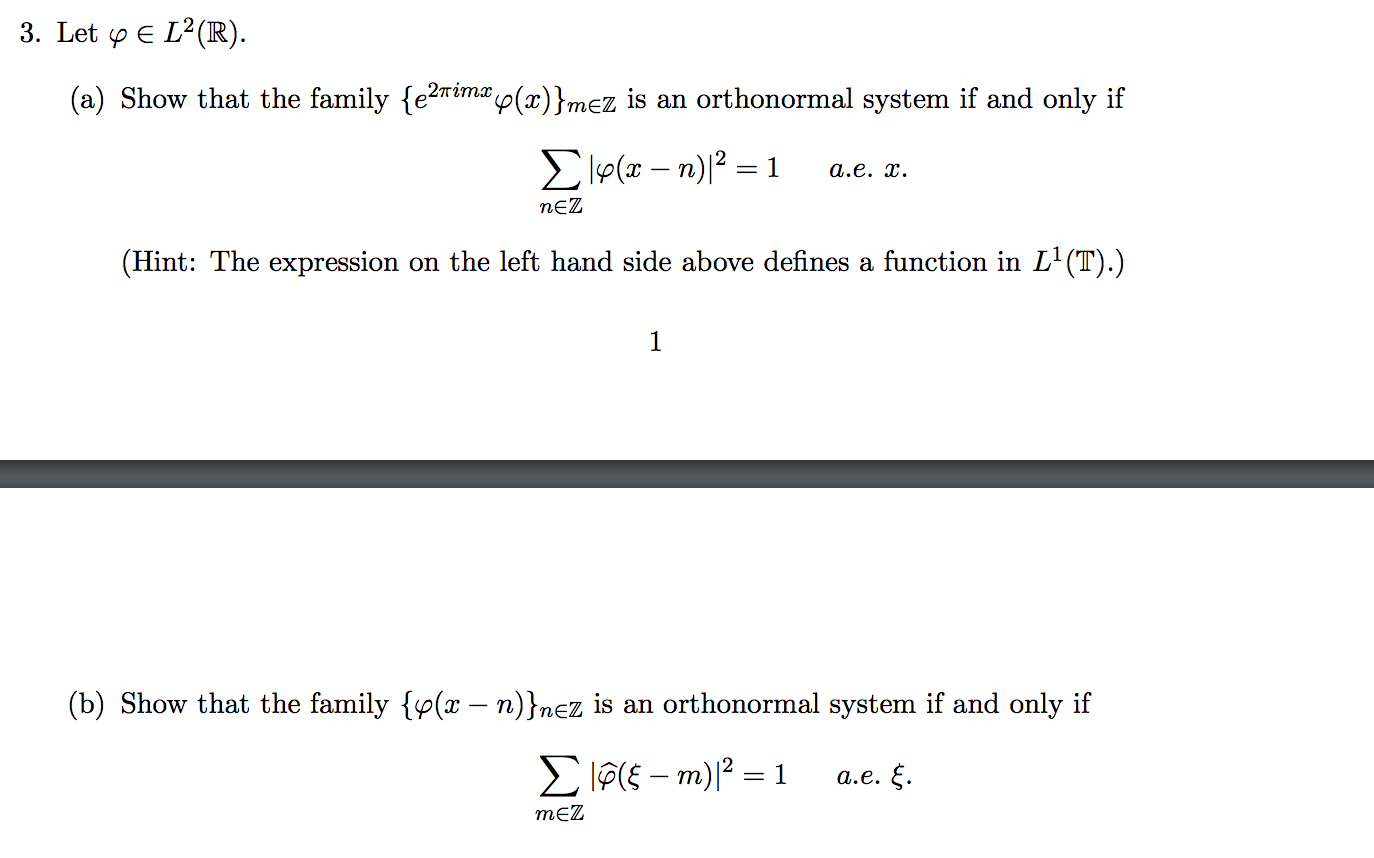
\includegraphics[width=0.8\textwidth]{HA-5-3.png}
\end{figure}
\end{question}
\begin{solution} \hfill \\

\textbf{(a)} We use the idea of periodization to prove both directions. 
For the converse, we compute, for any $n,m \in \mathbb{Z}$,
\eQb
<e_n \phi , \overline{e_m \phi} > &=& \sum_{k \in \mathbb{Z}} 
\int_{[0,1]-k} e^{2\pi i (n-m)x} |\phi(x)|^2 dx.
\eQe
With a change of variable $y = x + k$, the RHS of the above equality becomes
\eQb
\sum_{k \in \mathbb{Z}} \int_{0}^{1} e^{2\pi i (n-m)(y-k)} |\phi(y-k)|^2 dy, 
\eQe
which can be re-written as
\eQb
\int_{0}^{1} e^{2\pi i(n-m)y}\sum_{k \in \mathbb{Z}} |\phi(y-k)|^2 dy,
\eQe
and again be simplified to
\eQb
\int_{0}^{1} e^{2\pi i (n-m)y} dy,
\eQe
as the summand in the integral equals $1$ (absolutely convergent) by assumption and
$e_n$ is periodic to justify the interchange of the summand and the integral.
 With the last expression, we see that
$<e_n \phi, \overline{e_m \phi}>$ equals $1$ if $n = m$ and $0$ if $n \neq m$, which shows that
the given system is orthonormal. Now, for the forward direction, 
as $\phi \in L^2$, $|\phi|^2 \in L^1$,
we can set
\eQb
|\phi|_{\text{per}}^2 = \sum_{k \in \mathbb{Z}} |\phi(x-k)|^2.
\eQe
Taking a Fourier coefficient gives
\eQb
\widehat{|\phi|^2_{\text{per}}}(n) &=& \int_{\mathbb{T}} |\phi|_{\text{per}}^2 e^{-2\pi i n x} dx \\
&=& \int_{\mathbb{T}} \sum_{k \in \mathbb{Z}} |\phi(x-k)|^2 e^{-2\pi i nx } dx \\
&=& \int_{\mathbb{R}} |\phi(x)|^2 e^{-2\pi i nx} dx.
\eQe
By the orthornomral assumption, the above equality reveals that $\widehat{|\phi|^2_{\text{per}}}(n)$
is $1$ for the $0$th term and $0$ for the rest. Using the Cesaro convergence in $L^1$, we see that
\eQb
||1 - |\phi|^2_{\text{per}}|| = 0,
\eQe
which implie that $|\phi|_{\text{per}}|^2 = 1$ a.e., so by the established identity
\eQb
\sum_{k \in \mathbb{Z}} |\phi(x-k)|^2 = 1 \> \> \text{ a.e.},
\eQe
as required.

\textbf{(b)}
As $\varphi \in L^2$, we have $\hat{\varphi} \in L^2$. From $(a)$, it follows that
\eQb
\sum_{m \in \mathbb{Z}} |\hat{\varphi}(\xi-m)|^2 = 1 \> \text{ a.e. } \xi
\iff 
\{ e^{2\pi i m \xi} \hat{\varphi}(\xi) \}_{m \in \mathbb{Z}} \> \text{ is an ONS}.
\eQe
As the Fourier transform is an isometry on $L^2$, we have
\eQb
\{ \varphi(\xi -m)\}_{m \in \mathbb{Z}} \> \text{ is an ONS} 
\iff
\{ \widehat{\varphi(\xi-m)}\}_{m \in \mathbb{Z}} \> \text{ is an ONS},
\eQe 
which through the identity $\widehat{\varphi(\xi-m)} = \hat{\varphi}(\xi)e^{-2\pi i m\xi}$ 
and the first equivalence implies
\eQb
\sum_{m \in \mathbb{Z}} |\hat{\varphi}(\xi - m)|^2 = 1 \> \text{ a.e. } \xi 
\iff
\{\varphi(\xi -m )\}_{m \in \mathbb{Z}} \> \text{ is an ONS} 
\eQe
as required. \hfill $\qed$

\end{solution}

\newpage 

\begin{question}[4]
\hfill
\begin{figure}[h!]
  \centering
    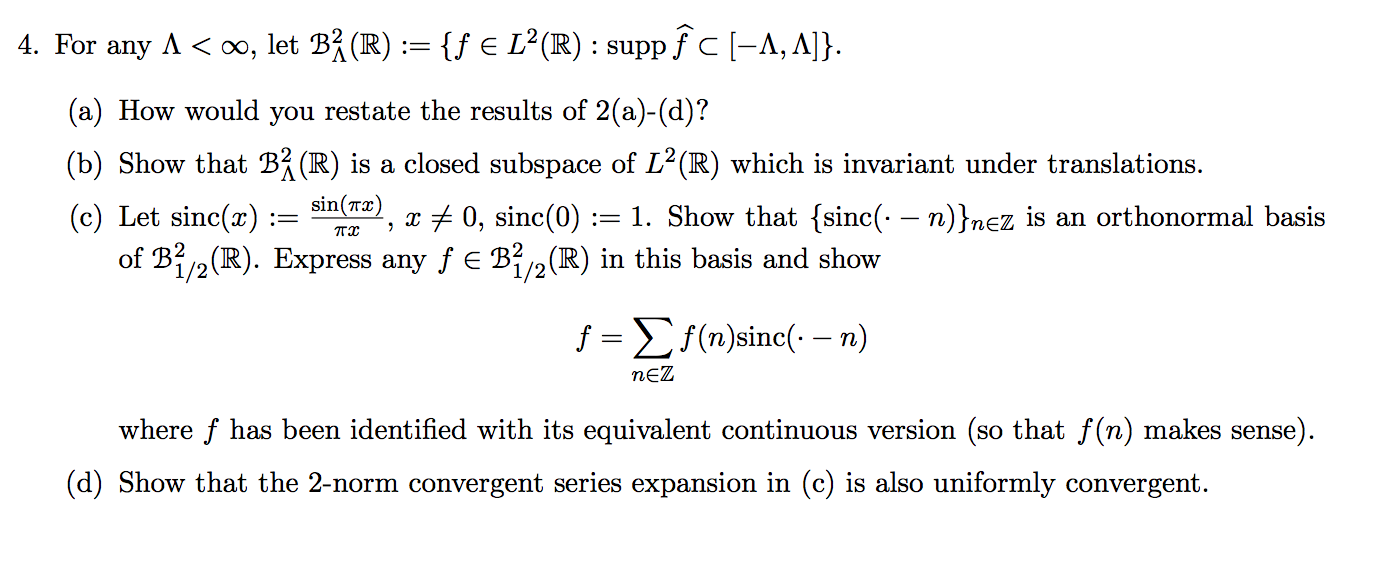
\includegraphics[width=0.8\textwidth]{HA-5-4.png}
\end{figure}
\end{question}
\begin{solution} \hfill \\
\textbf{(a)} We restate the results for $B^2_{\Lambda}$ instead of $B^1_{\Lambda}$,
but without changing the lower bound on $p$ from $1$ to $2$. 

\bigskip

\textbf{(b)} Let $\{f_n\}$ be a sequence in $B_{\Lambda}^2$ such that it converges to
some $f \in L^2$. As $||\hat{g}||_2 = ||g||_2$ for any $g \in L^2$, it follows that
$\{\hat{f_n}\}$ converges to $\hat{f}$ in $L^2$. Since the property of support being contained
in compact set
persists through $L^2$ limit (this trivially can be shown using a proof by contradiction), 
it follows that $\text{supp}\hat{f} \subset [-\Lambda,\Lambda]$,
so $f \in B_{\Lambda}^2$. Hence, $B_{\Lambda}^2$ is closed. 

\smallskip

We now show that $B_{\Lambda}^2$ is invariant under translations. Fix $h \in \mathbb{R}$, and
let $\eta_{h}$ be defined by $(\eta_{h}f)(x) = f(x-h)$ on $L^2$. Now, consider the modulation
operator $m_{h}$ to be defined by $(m_{h}f)(x) = e^{2\pi ih x}f(x)$. Then, it follows 
that, for $f \in L^2$, and $\xi \in \mathbb{R}$, 
\eQb
\widehat{\eta_{h}f}(\xi) &=& \int f(x-h)e^{-2\pi i \xi x} dx = (m_{-h}\hat{f})(\xi),
\eQe
so 
\eQb
\text{supp}\> \> \widehat{\eta_{h} f} = \text{supp}\> \> {m_{-h}}\hat{f} = \text{supp}
\>\> \hat{f}, 
\eQe
as one can trivially see that a support of a function is an invariant property under 
the modulation operator.
Therefore, we have shown that the translation operator is invariant on $B_{\Lambda}^2$.


\bigskip 

\textbf{(c)} 
Consider the space of functions defined by
\eQb
B_{\Lambda}^{2'} &=& \{ f \in L^2 \> | \> f(\xi) = 0 \> \text{ if } |\xi| > \dfrac{1}{2} \}.
\eQe
By Plancherel's theorem, the Fourier transform is a linear isometry from
$B_{\Lambda}^{2}$ to $B_{\Lambda}^{2'}$. We see that $\{e^{-2\pi i n \xi}1_{-(\frac{1}{2},\frac{1}{2}]}
\}$ is an orthonormal basis in $B_{\Lambda}^{2'}$. By the isometry relation, to show that the given
sinc set is an orthornal basis, it suffices to show that the the identified orthonormal basis is mapped to
sinc functions by inverse of the Fourier transform, which can be shown as
\eQb
F^{-1}(e^{-2\pi i n \xi })(x) &=& \int_{-\frac{1}{2}}^{\frac{1}{2}} 
e^{-2\pi i n \xi }e^{2\pi i \xi x} d\xi \\
&=& \text{sinc}(x -n), 
\eQe 
as required. 

Now, let $f \in B_{\Lambda}^{1}$ and $g = F(f)$. Using the basis identified, it follows that 
\eQb
g(\xi) &=& \sum_{n \in \mathbb{Z}} <g,e^{-2\pi i n \xi }> e^{-2\pi i n \xi}.
\eQe
Taking the inverse of the Fourier transform gives
\eQb
f(\xi) &=& \sum_{n \in \mathbb{Z}} <g,e^{-2\pi i n \xi}>\text{sinc}(\cdot -n),
\eQe    
which can be re-written as
\eQb
f(\xi) &=& \sum_{n \in \mathbb{Z}} f(n) \text{sinc}(\cdot -n),
\eQe
as $<g,e^{-2\pi i n \xi}> = f(n)$. Therefore, we are done.

\bigskip

\textbf{(d)} By Cauchy-Scwhwarz, it follows that
\eQb
\sum_{n \in \mathbb{Z}}|<f,\text{sinc}(\cdot-n)>||\text{sinc}(t-n)| &\leq& (\sum_{n \in \mathbb{Z}}
|<f,\text{sinc}(\cdot -n)>|^2)^{\frac{1}{2}} (\sum_{n \in \mathbb{Z}} \text{sinc}^2(t-n))^{\frac{1}{2}}. 
\eQe
In view of Parseval's theorem, we see that the first sum on the RHS converges, so
it suffices to show that the $\text{sinc}$ sum is uniformly bounded, but 
this can be shown with the comparison test with $\sum_{n \in \mathbb{Z}} \dfrac{1}{n^2}$. 
Therefore, the sum is uniformly bounded for all $t \in \mathbb{R}$, so the convergence is uniform by
Weistrauss M-test. \hfill $\qed$

\end{solution}

\end{document}
